
This section is devoted to the analysis and discussion of the results for our systematic mapping.
We proceed by \textit{(i)} presenting the collected data in a graphic form and \textit{(ii)} answering the research questions for our study.

%...............................................................................................................................................................
\subsection{Quantitative analysis}
%...............................................................................................................................................................
Our quantitative analysis of the results shows the  
frequencies of publications for each facet. Results have been aggregated in bullet charts (see  Figure~\ref{fig:publisherperyear}).
\begin{figure}
  \centering
  \subfloat[Publisher per Year]
  {\label{fig:publisherperyear}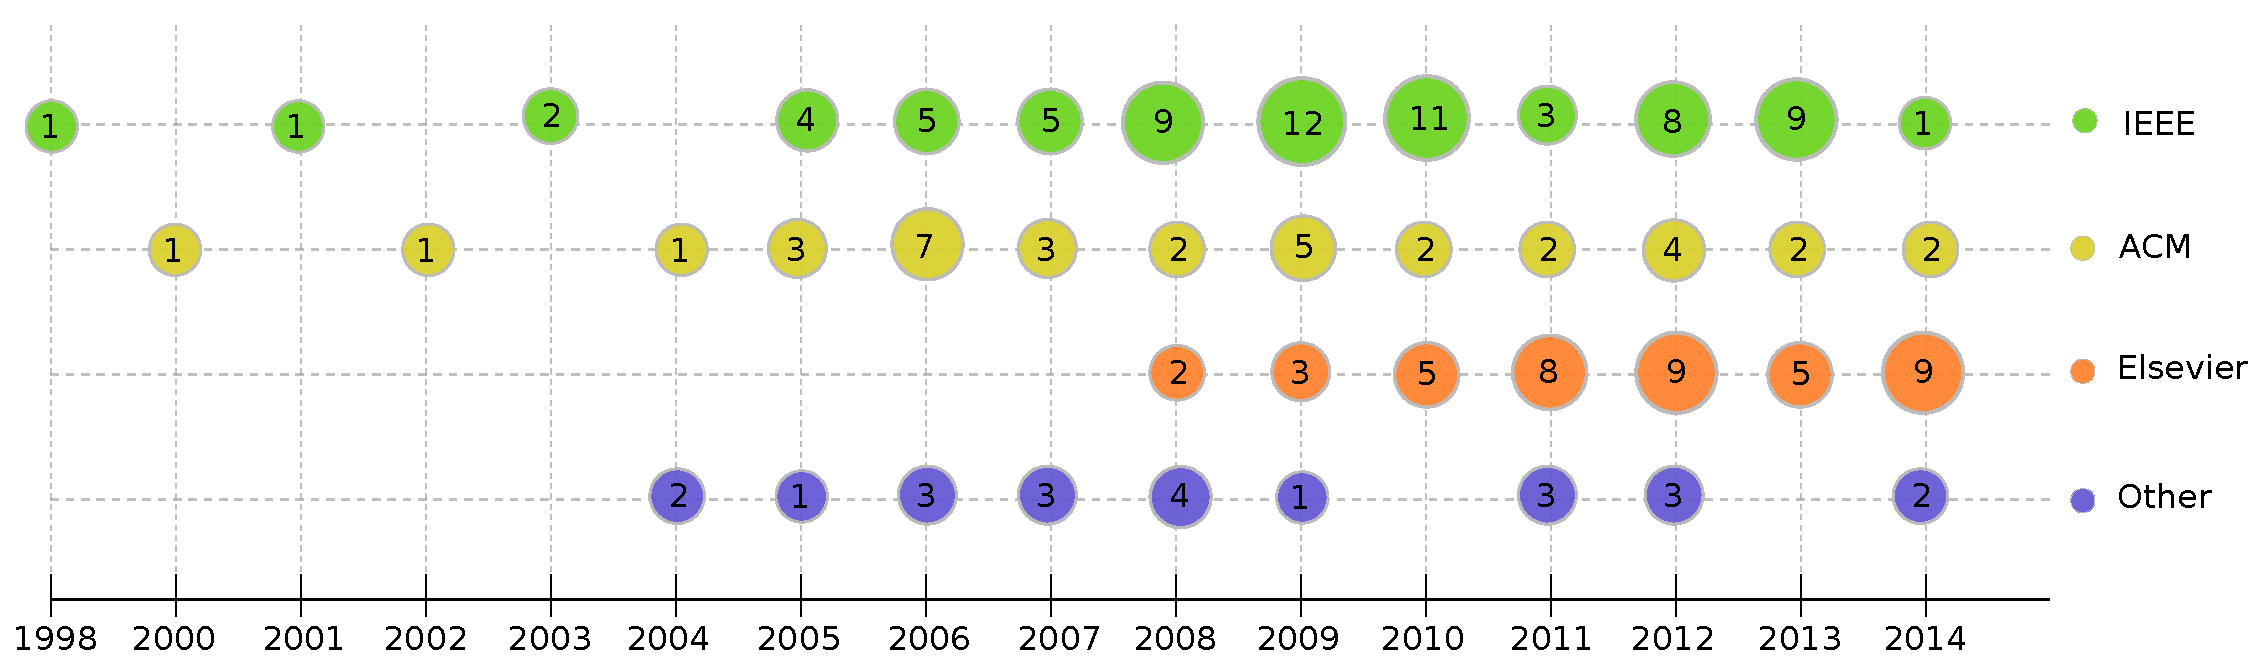
\includegraphics[width=0.99\textwidth]{figs/PublisherPerYear}}
  ~ %add desired spacing between images, e. g. ~, \quad, \qquad etc. (or a blank line to force the subfig onto a new line)
  \\
  \subfloat[Contribution per Year]
  {\label{fig:contributionperyear}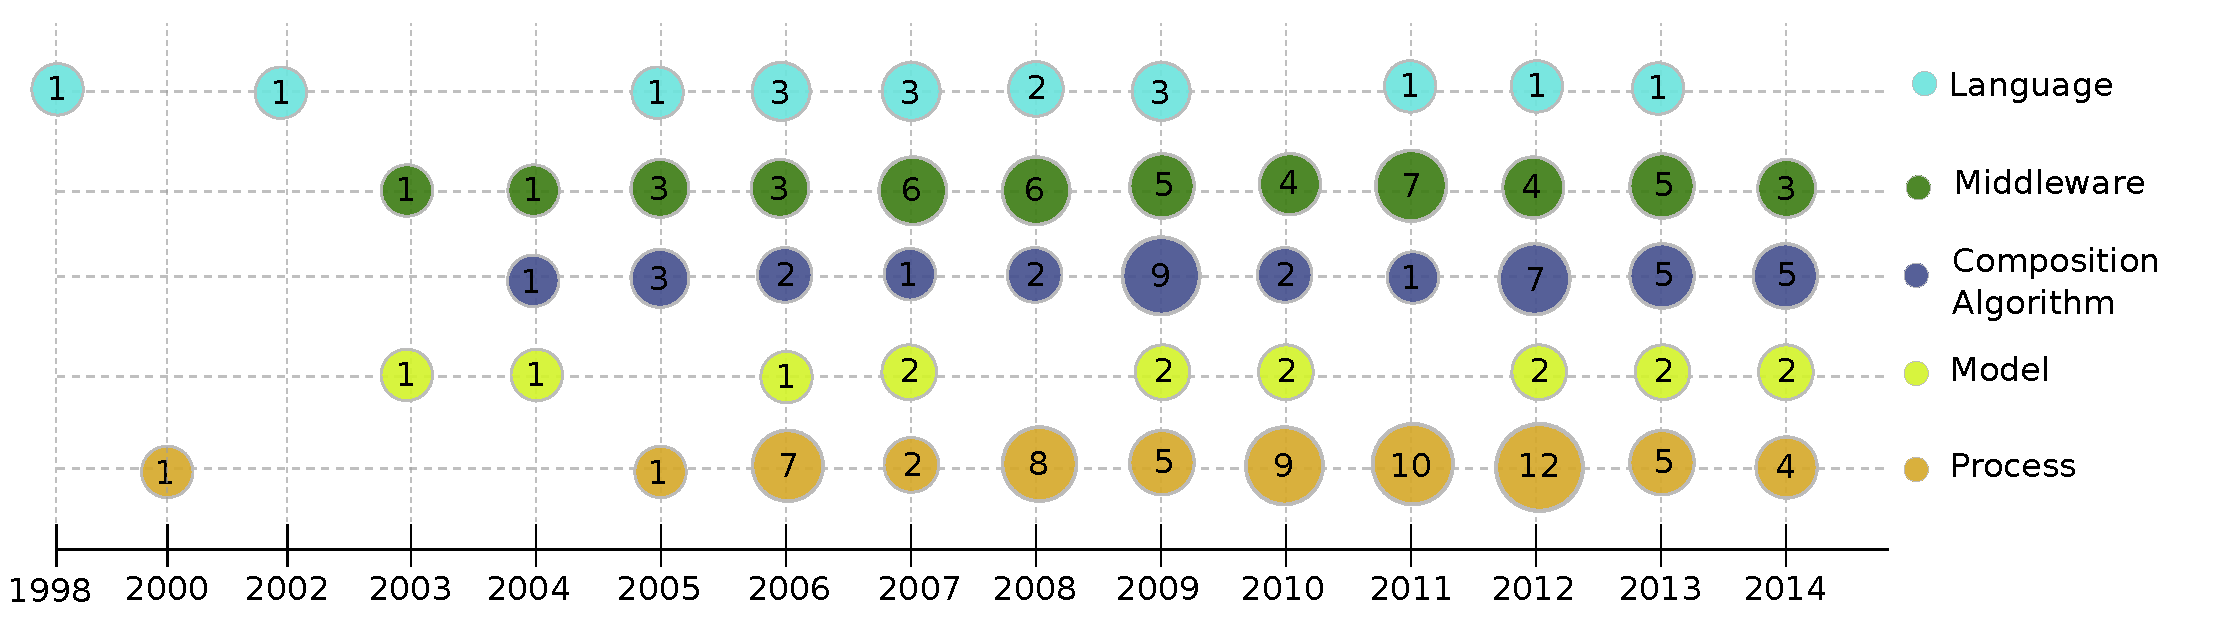
\includegraphics[width=0.99\textwidth]{figs/ContributionPerYear}}
   %add desired spacing between images, e. g. ~, \quad, \qquad etc. (or a blank line to force the subfig onto a new line)
  ~
  \\
  \subfloat[Paradigm per Year]
  {\label{fig:paradigmperyear}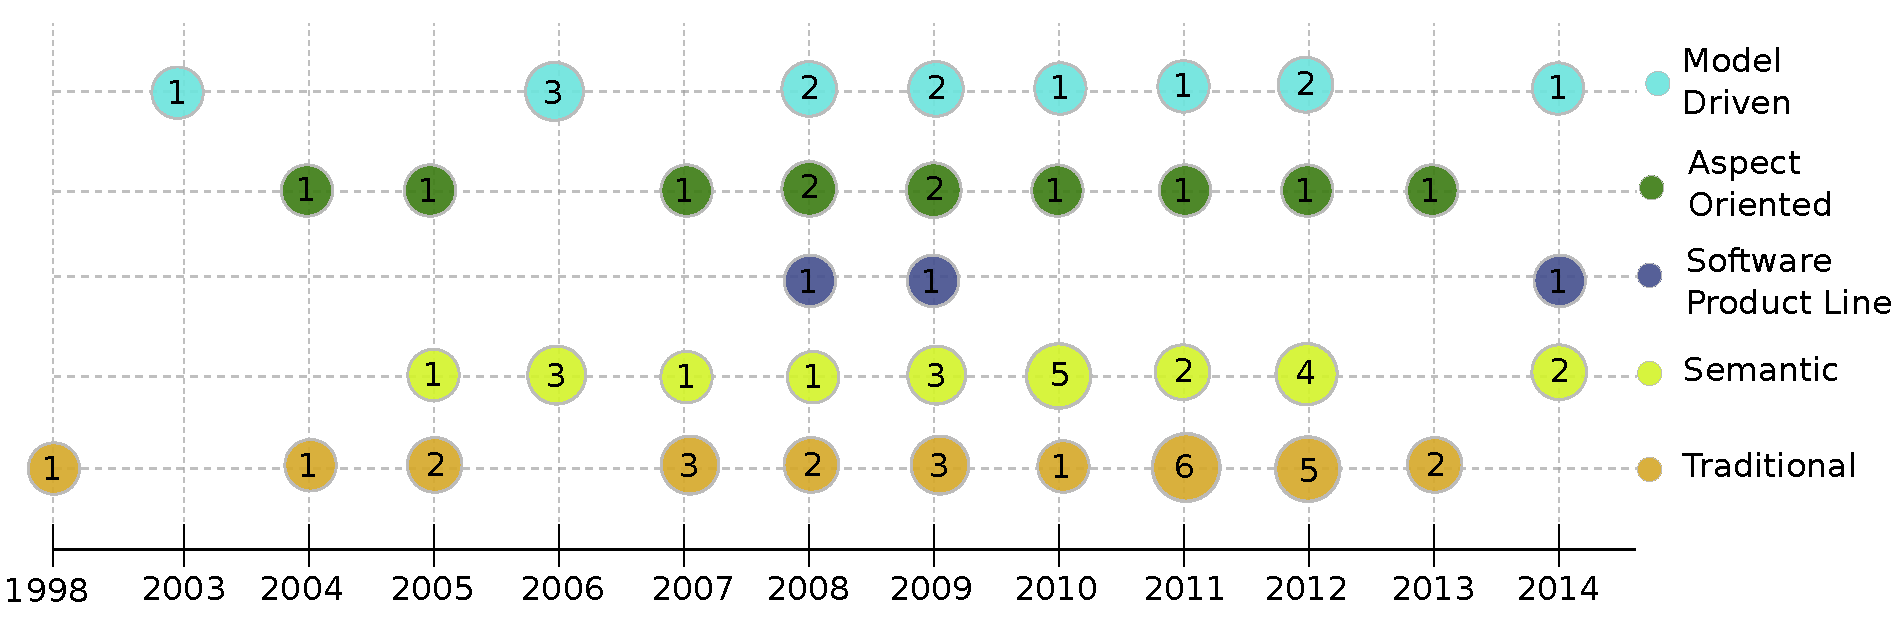
\includegraphics[width=0.99\textwidth]{figs/ParadigmPerYearNew}}
  ~ %add desired spacing between images, e. g. ~, \quad, \qquad etc. (or a blank line to force the subfig onto a new line)

  \caption{Publications per Year}
  \label{fig:publicationsperyear}
\end{figure}

We computed bubble charts that aggregate the number of papers published by year in the area (see
Figure \ref{fig:publicationsperyear}).  The following  presents the aggregated view of the number of papers published by year and by facet.

Despite  the low number of works tackling \textit{other} publishers, they
maintain their presence over the years,  mainly between 2008-2014. IEEE and ACM are
the publishers that most published papers related to service-oriented
applications considering non-functional properties. Considering Elsevier, we can
found papers only from 2008. Figure \ref{fig:publisherperyear} presents the
publications for each publisher per year.    

Figure \ref{fig:contributionperyear} presents the distribution of papers per
contribution category by year. As shown in the figure, particularly between 2008 and 2012 most papers propose a middleware and a process, while composition algorithms were mainly published in 2008 and 2012. Papers proposing \textit{SPL} are not numerous but the number remains stable along the years, while semantic and traditional proposals are quite popular.

 
 %......................................................................................
\subsection{Analysis by combining facets}
%......................................................................................
For the analysis, we computed the
volume of publications by publisher (Figure \ref{fig:publisherperyear}). We
also analyzed the publications considering the facets 
{\em contribution} and {\em paradigm} as pivot references that can be then put in perspectives by combining them with the other three facets (see Figures \ref{fig:contributionperyear} and
\ref{fig:paradigmperyear}).
The facet contribution   serves to organize papers that propose solutions for modelling, expressing and implementing NFR for service-based applications (Figures
\ref{fig:Facets-Contribution-ProcessParadigm}, 
\ref{fig:Facets-Contribution-MatematicalModel} and
\ref{fig:Facets-Contribution-NFR}). The facet paradigm serves to organize papers that propose methodologies for implementing service based software with  NFR (Figure \ref{fig:Facets-Paradigm-ContributionProcess}). 

%......................................................................................
\subsubsection{Contribution - Process - Paradigm facets}
%......................................................................................
\begin{figure} [htpb]
\centering
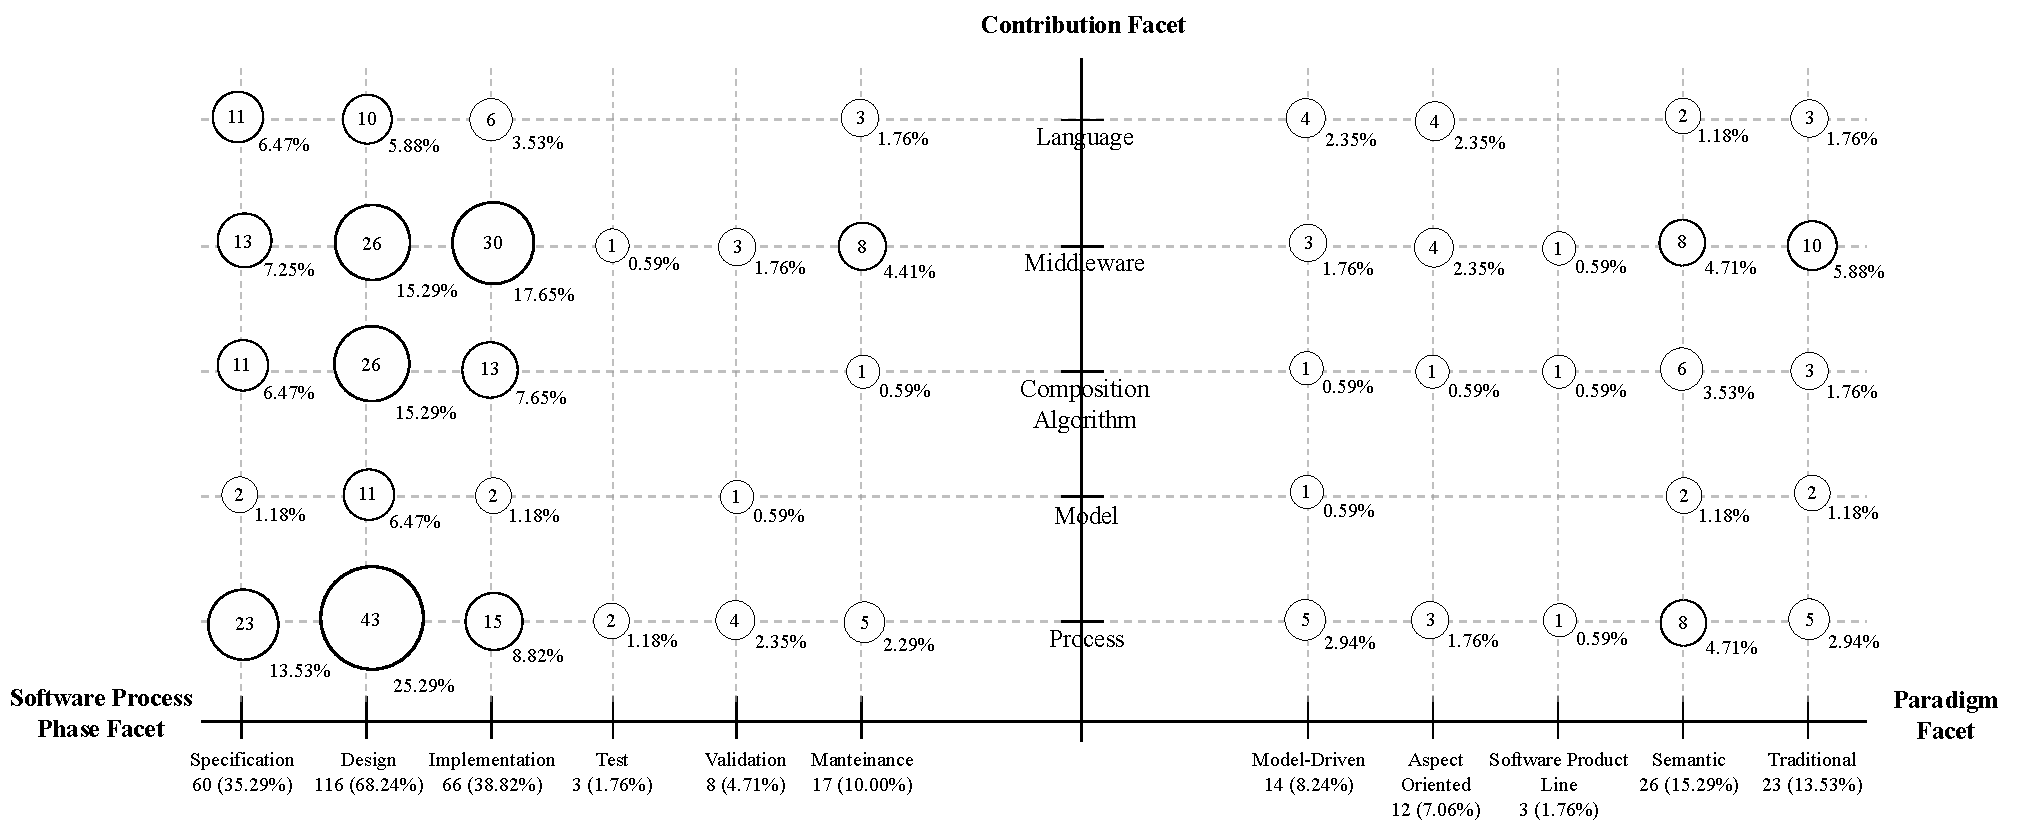
\includegraphics[width=0.99\textwidth]{figs/Facets-Contribution-ProcessParadigm}
\caption{Facet Contribution with facets Software development process and Paradigm }
\label{fig:Facets-Contribution-ProcessParadigm}
\end{figure}   

We combined the facet {\em contribution} with the facets {\em process} and {\em paradigm} to try to observe the relationship between the contribution associated to software development phase and the type of contribution reported in a paper (see
Figure
\ref{fig:Facets-Contribution-ProcessParadigm}). We observed that NFR are rarely considered in the test, validation and maintenance phases of a service-based software development methodology. There are 8 papers that relate
middleware (contribution) with the maintenance phase in their  proposals. 
Specification (35.29\%), Design (68.24\%) and Implementation
(38.82\%)\footnote{There are papers which were classified in more than one
category, considering all facets, \textit{e.g.}, one paper may be classified
in design and implementation; or middleware and composition algorithm.} are the phases most frequently addressed in papers.
Papers addressing the design phase of the service-based software development is the that has almost all categories of contributions defined in our facet. Yet, fewer consider middleware and language as adapted contributions for addressing NFR in these phases.
Middleware proposals focus on the implementation phase in 30
papers (17.65\%), and 26 papers (15.29\%) on the design phase. Languages seem to be well adapted for expressing NFR in the specification  (11 works -6.47\%), and design phases (10
works 5.88\%). The majority of
papers  proposing a Process in the Contribution facet (53.46\%) are related to the
categories of the facet software process phase).  

Associating the facets contribution and paradigm we observed that there are
few works  (1.76\% ) that use Software Product Line to propose some kind of contribution for 
 service-based
software with NFR.  Semantic and traditional paradigms are almost systematically used when papers propose a
 Middleware and a Process. Works that propose a composition
algorithm are almost always related to at least one of the paradigm categories.
       
%......................................................................................
\subsubsection{Combining facets Contribution and Mathematical Model}
%......................................................................................
 \begin{figure}[ht!]
\centering
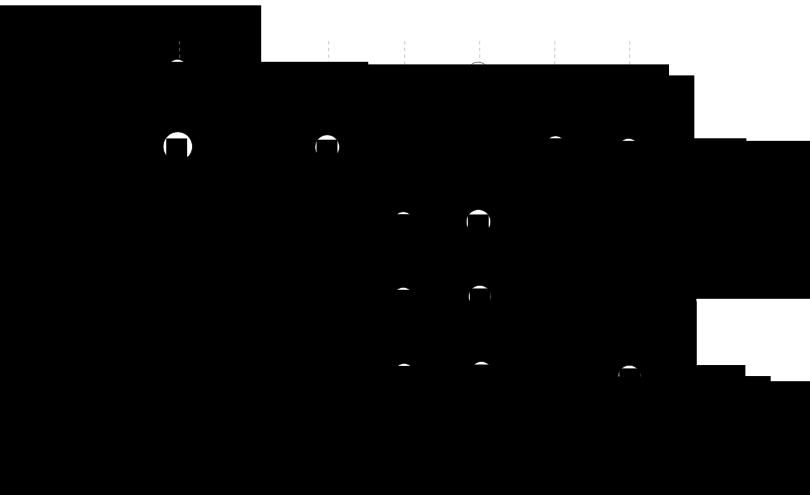
\includegraphics[width=0.99\textwidth]{figs/Facets-Contribution-MatematicalModel}
\caption{Contribution and Mathematical Model Facets}
\label{fig:Facets-Contribution-MatematicalModel}
\end{figure}   

We combined the facets {\em Contribution} and {\em Mathematical model} to determine which formal tool has been used the most to define different types of contributions (i.e., languages, models, methods), or whether there is a generic formal tool used for all types of contributions (Figure \ref{fig:Facets-Contribution-MatematicalModel}). We observed that contributions proposing algorithms  or processes for automatizing service composition use in general  heuristics or optimization category (55 papers -32.35\%). The majority of the contributions proposed composition algorithms (21 papers -12.35\%) and processes  (22 -12.9\%). The majority of contributions proposing Middleware and Process use  Petri Nets, Automata and Agents. Only 2 papers (1.18\%) propose new languages for
service-based software with NFR. 
 
 %......................................................................................
\subsubsection{Combining the facets Contribution and NFR type}
%......................................................................................

\begin{figure}[ht!]
\centering
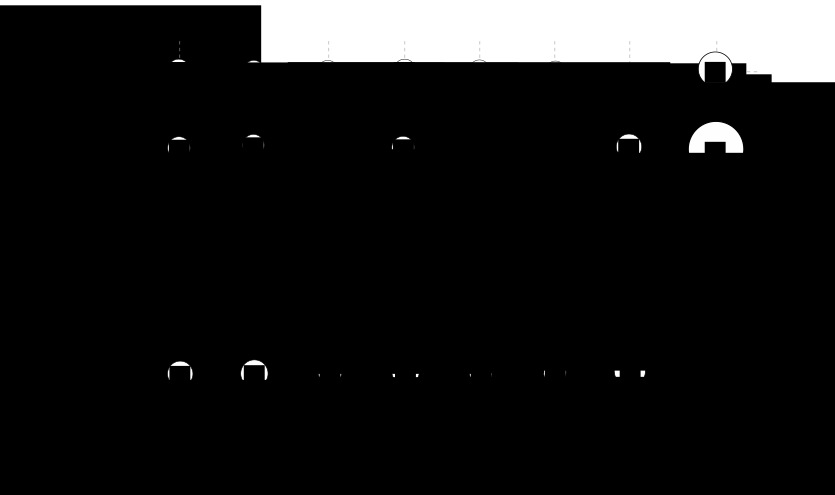
\includegraphics[width=0.99\textwidth]{figs/Facets-Contribution-NFR}
\caption{Facets Contribution and NFR Type}
\label{fig:Facets-Contribution-NFR}
\end{figure}  
       
We combined the facets {\em Contribution} and {\em NFR type} to observe the papers that (i) report solutions concerning all NFR types o just particular ones for service-based software; and (ii) the contributions that are used the most for specific NFR types (see
Figure \ref{fig:Facets-Contribution-NFR}).  First, with respect to the type of NFR, the proposals concerning general solutions that address NFR as a type of QoS are very popular (129/170papers -75.88\%). Quality properties are expressed and associated to service compositions. There are few proposals that address other NFR types  (e.g., Usability, Maintainability, Portability, Functionality, Reliability and Efficiency). Only 15 works (8.82\%) address one of
these NFR types. 

%......................................................................................
\subsubsection{Combining the facet Paradigm with the facets Contribution  and Software process development}
%......................................................................................
\begin{figure} [htpb]
\centering
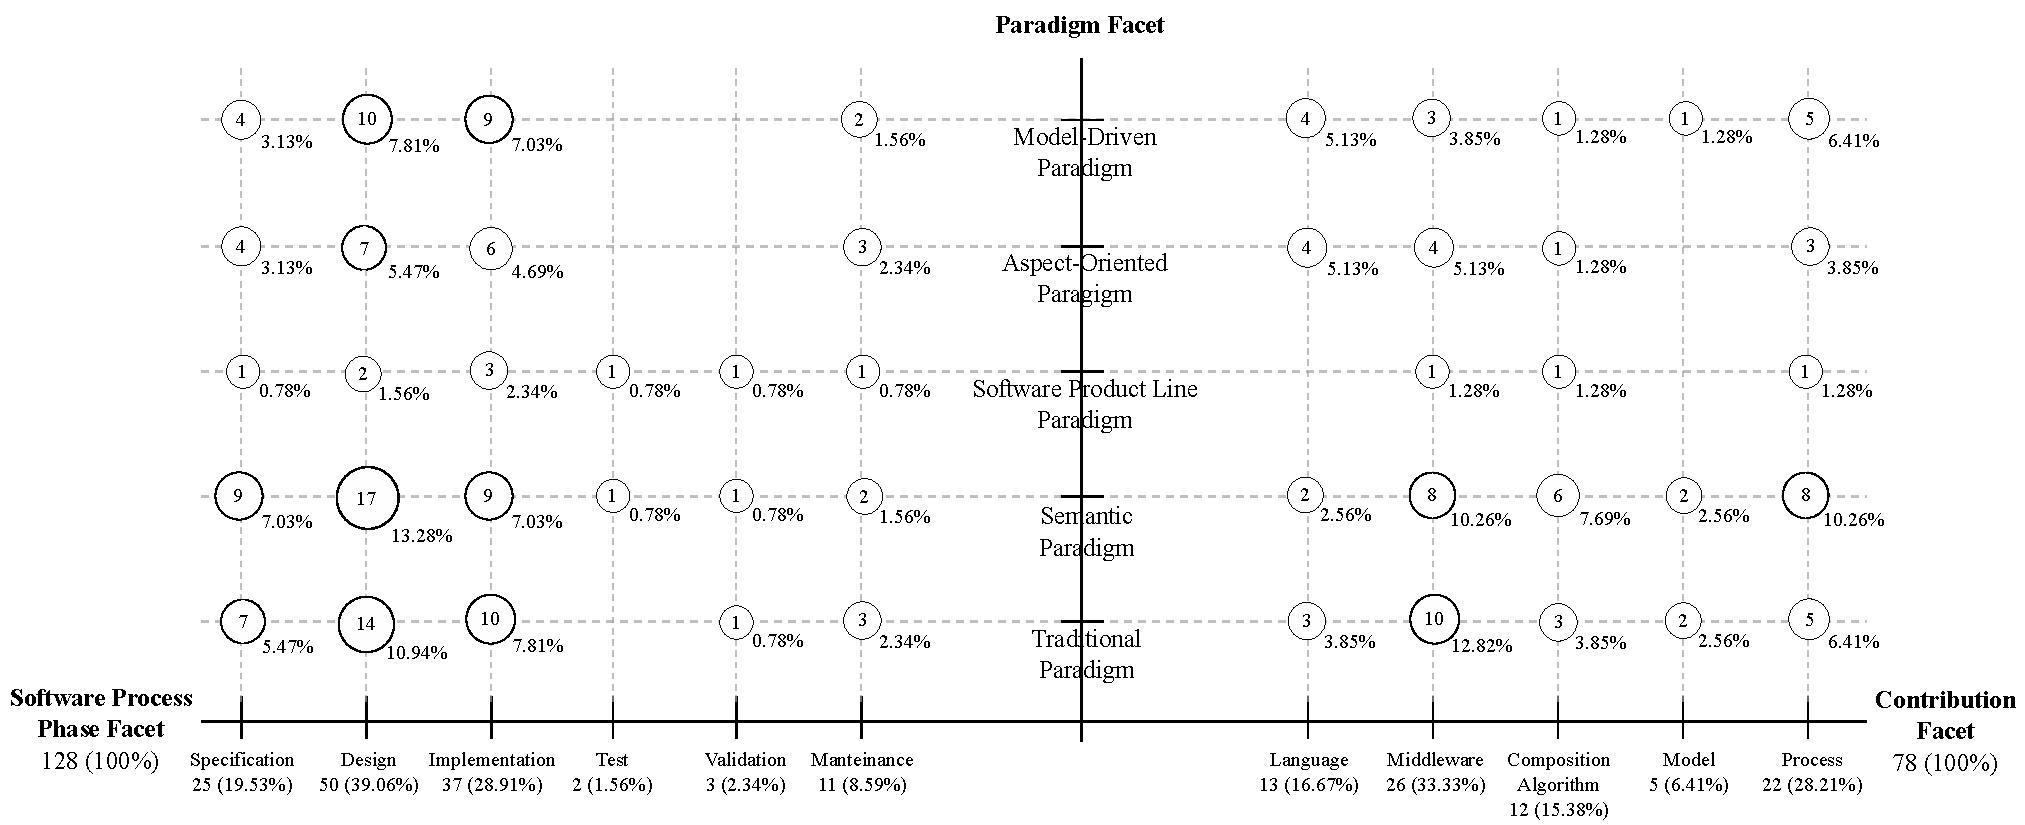
\includegraphics[width=0.99\textwidth]{figs/Facets-Paradigm-ContributionProcess}
\caption{Paradigm and Contribution/Process Facets}
\label{fig:Facets-Paradigm-ContributionProcess}
\end{figure}  

Combining the facet Paradigm with the facets Contribution and Software process development (Figure
\ref{fig:Facets-Paradigm-ContributionProcess})  it is possible to observe the phases in which software methodologies contribute to address NFR for service-based software. We also  observed whether there is a connexion between the paradigm used by methodologies with respect to the way the address NFR.
First of all, the most popular paradigms adopted by software development methodologies are Semantic with 17 papers (13:28\%), Model-Driven Development with
10 papers (7.81\%) and Traditional paradigm with 14 works (10.94\%). 
Second, the analysis shows that the phases Test and Validation are rarely addressed by methodologies independently of the adopted paradigm (2 papers for Test and 3 for Validation). In contrast, the Design, Specification and Implementation phases are addressed by a lot of methodologies independently of the adapted paradigm.
 
 %The relationship between Paradigm and the Contribution was made in the
%description of Figure \ref{fig:Facets-Contribution-ProcessParadigm}.

%......................................................................................
%\subsubsection{Combining the facets Paradigm and Mathematical Model}
%......................................................................................

%\begin{figure} [htpb]
%\centering
%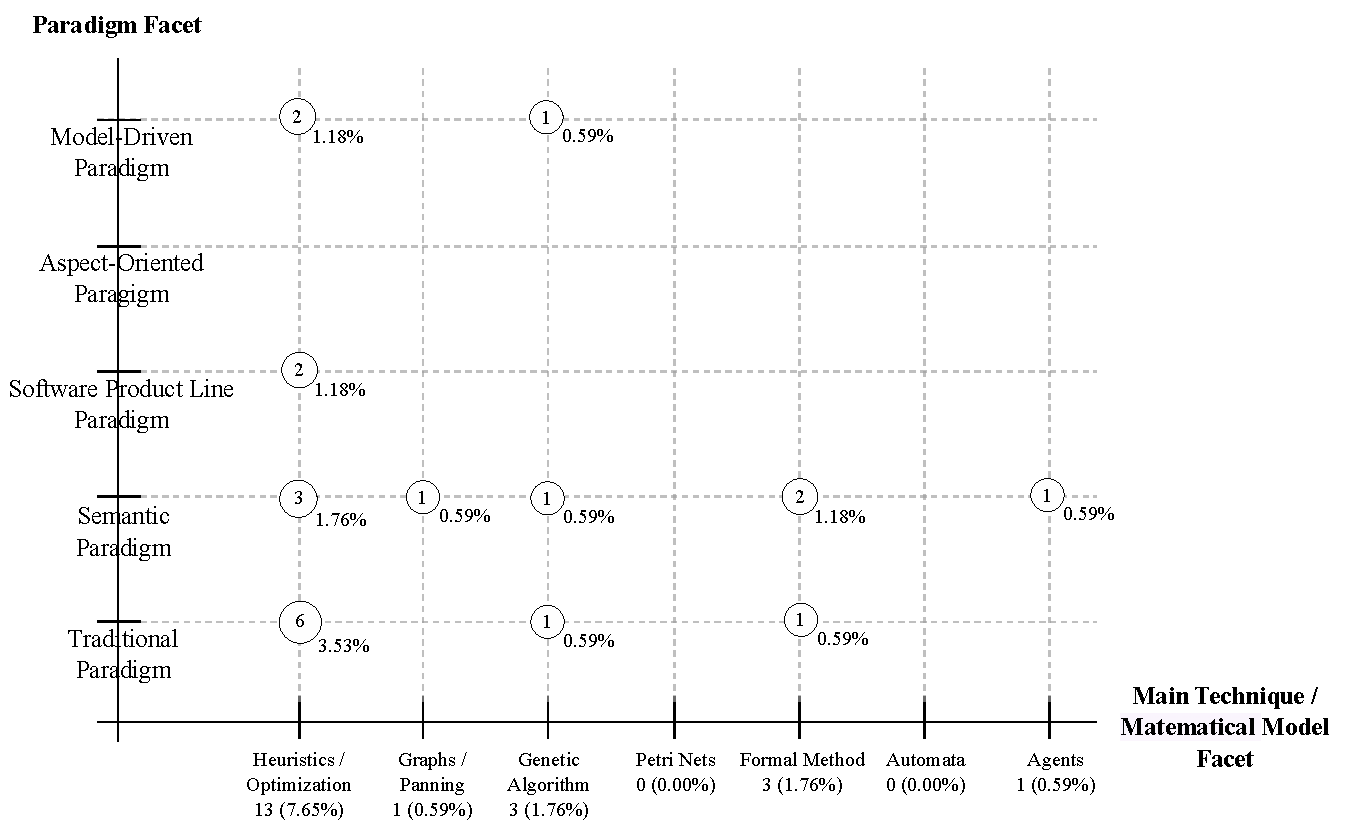
\includegraphics[width=0.9\textwidth]{figs/Facets-Paradigm-MatematicalModel}
%\caption{Paradigm and Matematical Model Facets}
%\label{fig:Facets-Paradigm-MatematicalModel}
%\end{figure}   


%Considering Figures \ref{fig:Facets-Paradigm-MatematicalModel} and
%\ref{fig:Facets-Paradigm-NFR} we can see some gaps in the relation of the
%Paradigm used and the Main Technique/Matematical Model or the NFR type
%presented. This result occurs because 76 paper, among them 170 (44.70\%)
%selected after the systematic mapping filters, could be classified in one the
%five categories of the Paradigm facet. Thus, from this point of view, there are
%some empty intersection points. For example, in Figure
%\ref{fig:Facets-Paradigm-MatematicalModel} and considering the Aspect-Oriented
%line, there is no paper which uses a mathematical model to solve problems related
%with service-based approaches in the presence of non-functional requirements.
%From Software Product Line, only two papers addresses Heuristic /
%Optimization. By one other hand, Semantic is the most used Paradigm in this
%context, representing only 4.71\% of the papers. By the other hand, the
%works which considers Semantic does not have relation with those that uses
%Petri Nets and Automata.

%......................................................................................
%\subsubsection{Combining the facets Paradigm with NFR}
%......................................................................................
%\begin{figure} [htpb]
%\centering
%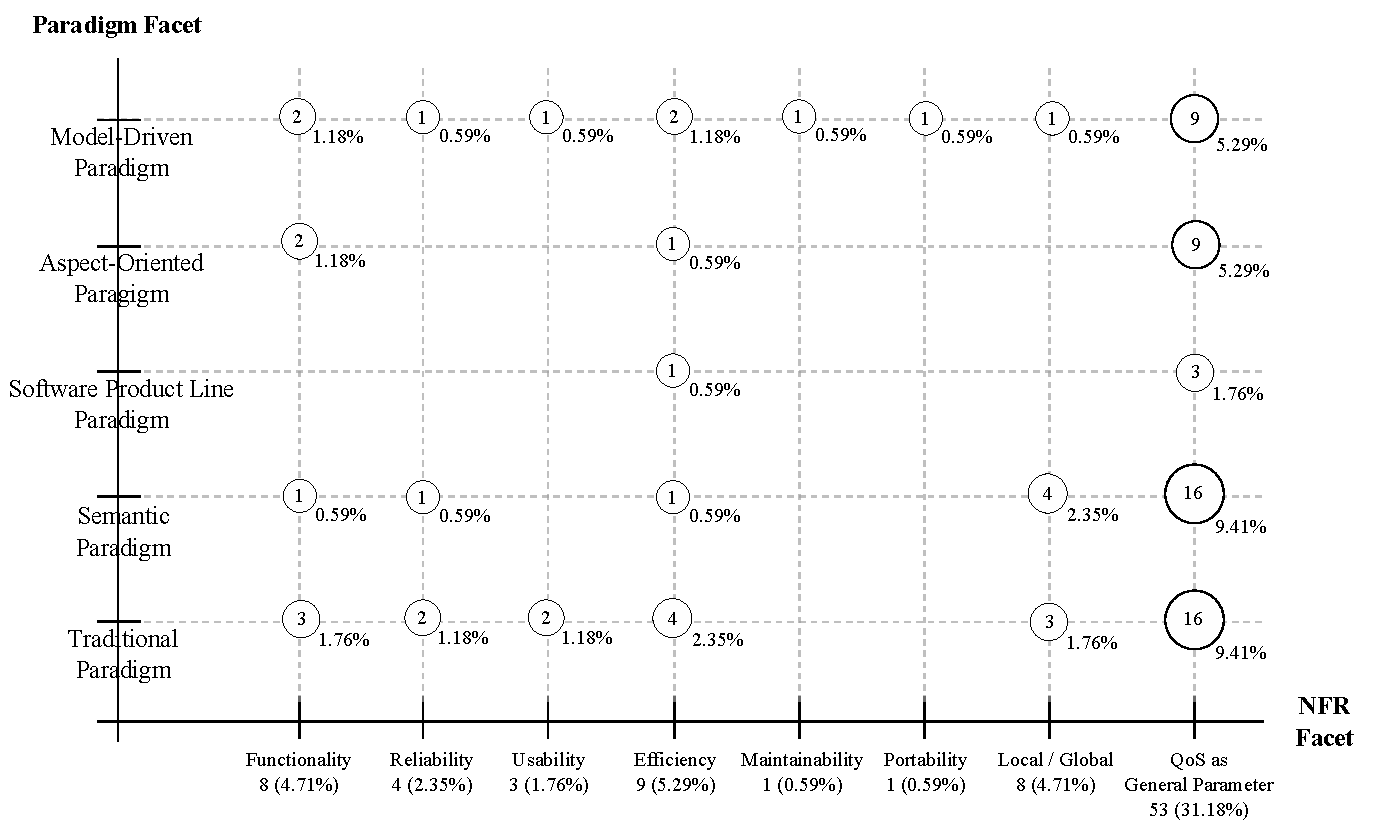
\includegraphics[width=0.9\textwidth]{figs/Facets-Paradigm-NFR}
%\caption{Paradigm and NFR Type Facets}
%\label{fig:Facets-Paradigm-NFR}
%\end{figure}   

%In Figure \ref{fig:Facets-Paradigm-NFR} we can see as similar as Figure
%\ref{fig:Facets-Contribution-NFR}, Usability, Maintainability
%and Portability are the NFR categories with less number of proposals from the
%perspective of the Paradigm facet and also the service-based composition domain.
%Eficiency and QoS are the two categories related with all Paradigm categories.
%Although, the most paper (53, representing 31.18\%) are classified using QoS.
%From these, Semantic and Traditional paradigms are the most frequent used. 
 


 